\documentclass[tikz]{standalone}
\def\surroundcircle{(0,0) circle (4)}
\def\firstcircle{(90:1.2) circle (2)}
\def\secondcircle{(210:1.2) circle (2)}
\def\thirdcircle{(330:1.2) circle (2)}
\begin{document}
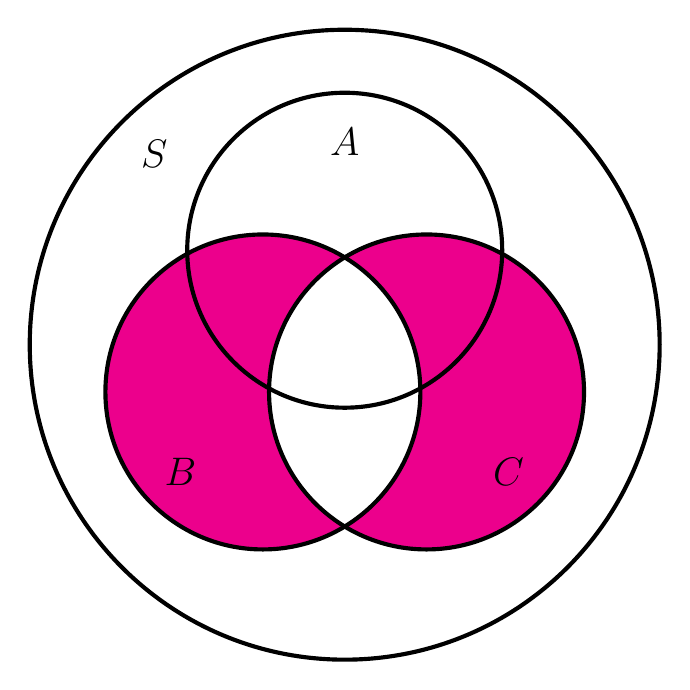
\begin{tikzpicture}
\begin{scope}[blend group=soft light]
  \fill[even odd rule, magenta] \secondcircle \thirdcircle;
\end{scope}
\begin{scope}[line width=1.5pt, font=\Large]
  \draw \firstcircle node [text=black,above=30] {$A$};
  \draw \secondcircle node [text=black,below left=20] {$B$};
  \draw \thirdcircle node [text=black,below right=20] {$C$};
  \draw \surroundcircle node [text=black,above left=60] {$S$};
\end{scope}
\end{tikzpicture}
\end{document}
